\section{My Research}

\begin{frame}{Hyperplane Arrangements}

    \begin{itemize}
       \item What if we included both sides of each hyperplane?
       \item Get something unbounded\footnote{Corresponding to \emph{``hypertoric manifolds''}.}.
    \end{itemize}

    \begin{figure}
        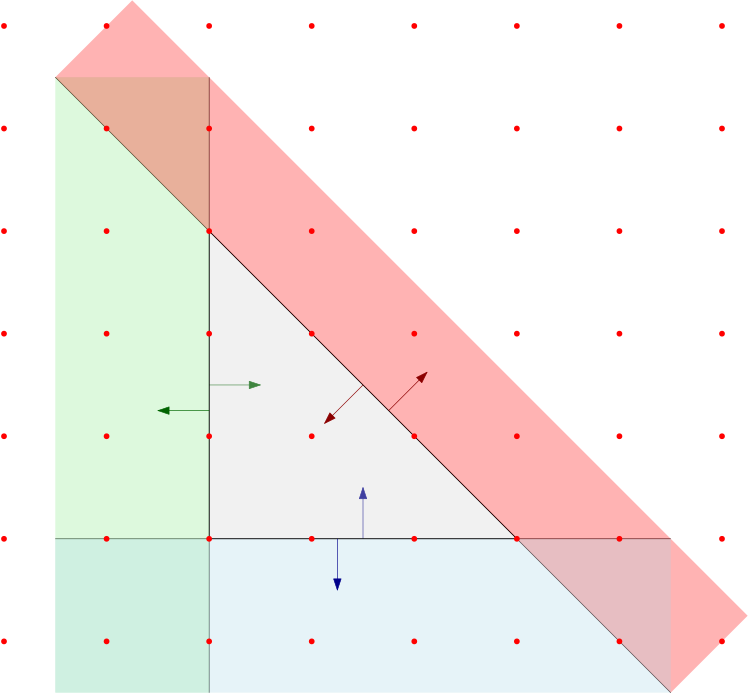
\includegraphics[scale=0.2]{resources/hyperplanes.png}
    \end{figure}

\end{frame}

\begin{frame}{Quantisation?}

    \begin{itemize}
       \item But now, $\#$ lattice points $= \infty$!
       \item Compactify the arrangement into a \emph{``polyptych''}\footnote{Coined by J. Martens.}.
    \end{itemize}

    \begin{figure}
        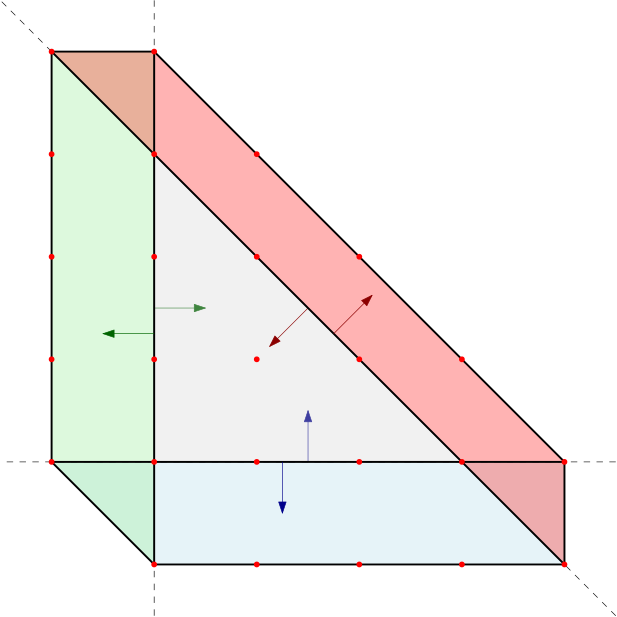
\includegraphics[scale=0.2]{resources/polyptych.png}
    \end{figure}

\end{frame}